\documentclass[10pt]{article}
\usepackage[utf8]{inputenc}
\usepackage[spanish]{babel}
\usepackage{url}
\usepackage{hyperref}
\usepackage{amsmath}
\usepackage{amsfonts}
\usepackage{amssymb}
\usepackage{graphicx}
\usepackage{float}
\usepackage{lipsum}
\usepackage{multicol}
\usepackage{xcolor}
\usepackage{braket}
\usepackage{cancel}
\usepackage[T1]{fontenc}
\usepackage{array}
\usepackage{booktabs}
\newcommand{\celda}[1]{
	\begin{minipage}{2cm}
		\vspace{5mm}
		#1
		\vspace{5mm}
	\end{minipage}
}
\definecolor{verde}{rgb}{0.24, 0.58, 0.26}
\usepackage[left=1cm, right=1cm, top=2cm, bottom=2cm]{geometry}
\author{Nelson David Forero Martínez}
\title{Didáctica de Probabilidad y Estadística}

\begin{document}

	\begin{figure}[H]
		\centering
	 
\includegraphics[scale=0.15]{udlogo.png}
	\end{figure}

%	\vspace{1.5mm}%
	
	\begin{center}
		{\Large \textbf{Muestreo Aleatorio Estratificado}}\\
		{\large Forero Martínez Nelson David}
				\vspace{0.5mm}\\
		$^1$ndforero4@gmail.com, \textit{Facultad de Ciencias y Educación.}  \\ \textit{Análisis Estadístico Utilizando RStudio}\\
						\vspace{2mm}
		\end{center}

	\begin{center}
		\textcolor{black}{\rule{200mm}{0.5mm}}
	\end{center}		

	
		\section*{Introducción} 
             
       El muestreo aleatorio estratificado es una técnica de muestreo probabilístico en la que se divide una población en diferentes subgrupos o estratos. Cada estrato está compuesto por individuos que comparten características similares. La muestra se selecciona de manera proporcional en cada estrato, lo que garantiza que la muestra represente adecuadamente los subgrupos específicos de la población. 
       
       Así pues, en el presente informe se realiza un Muestreo Aleatorio Estratificado a partir de una base de datos que compara el precio que pagan ciudadanos de cuatro ciudades de Colombia por los servicios púbicos. También se hallarán las siguientes variables: Estimacion de la media, la Varianza, el Intervalo de confianza para la media, el Intervalo de confianza, la Estimación del error, la  Estimación del total, la Estimacion de la Proporcion, la Cota de error para la proporción y el Intervalo de confianza para la proporción en el MAE, todo ello a partir del aplicativo de RStudio. 

             
		\subsection*{Presentación}

        En una muestra aleatoria estratificada se divide la población en estratos que son porciones disyuntas de la población y posteriormente se selecciona una muestra aleatoria simple de cada uno de esos estratos. De tal manera, la probabilidad de que dos elementos estén en el mismo estrato es nula, es decir, igual a cero. 

        Así pues, la base de datos con la cual se trabajará es una base de en donde se muestra el valor que pagan los ciudadanos por los servicios públicos en 4 ciudades, las cuales serán consideradas como los estratos, así el estrato 1 será Bogotá, el estrato 2 será Cali, el estrato 3 será Medellín y el estrato 4 será Cartagena. 
                   
        \subsection*{Aproximación al tamaño de muestra en el muestreo aleatorio estratificado para estimar la media aritmética}

        Para hallar el tamaño de la muestra en el muestreo aleatorio estratoficado, primero es necesario calcular el total de observaciones $(N)$ y luego el total de observaciones por estrato. De esta manera, el modelo multiplica el tamaño del estrato (o población) por la desviación estándar del estrato y se divide por los costos del estráto i-ésimo, y se hace así para cada uno de los estratos. 

        $$
        n=\frac{  \left ( \frac{N_1\sigma _1}{\sqrt{c_1}} + \frac{N_2\sigma _2}{\sqrt{c_2}}+...+\frac{N_L\sigma _L}{\sqrt{c_L}}\right )\left ( N_1 \sigma _1 \sqrt{c_1}+N_2 \sigma _2 \sqrt{c_2}+...+N_L \sigma _L \sqrt{c_L}\right )}{N^2\frac{E^2}{4}+\left ( N_1 \sigma^2 _1 +N_2 \sigma^2 _2 +...+N_L \sigma^2 _L \right )}
        $$

        Donde 

        \begin{itemize}
            \item $N_1 \to$ es el número de elementos en el estrato l-ésimo.
            \item $N \to$ es el número total de datos $N_1+N_2+...+N_L$.
            \item $\sigma_i \to$ es la desviación estándar del estrato i-ésimo.
            \item $c_i \to$ costos de realizar una encuesta en el estrato i-ésimo.
        \end{itemize}

        De esta manera, se tiene que hallar el valor $N$ que es el número total de datos $N_1+N_2+...+N_L$, haciendo uso de RStudio se tiene que $N=6849$. Dicho dato se obtiene a sumar los estratos de Bogotá, Cali, Medellín y Cartagena. 

         \begin{figure}[H]
                	\centering
                    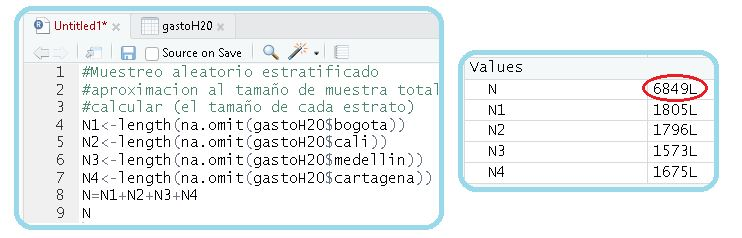
\includegraphics[scale=0.6]{Est1.JPG}
                    \caption{Tamaño de los estratos en RStudio}
                    \label{etiqueta1}
            \end{figure}

        A continuación, se hallará la desviación estándar por estrato haciendo uso de RStudio. Se obtenie que $\sigma _1=202.3$, $\sigma _2=175.9$, $\sigma _1=143.7$ y $\sigma _1=230.1$.

            \begin{figure}[H]
                	\centering
                    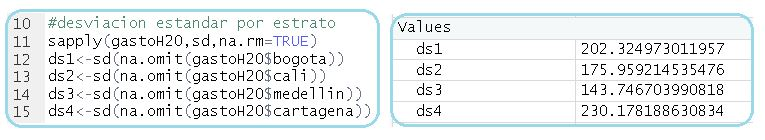
\includegraphics[scale=0.6]{Est2.JPG}
                    \caption{Desviación estándar por estratos en RStudio}
                    \label{etiqueta2}
            \end{figure}
        
        Seguidamente, estipulan los costos de realizar una encuesta en el estrato i-ésimo. Se tiene que $c_1=3000$, $c_2=2500$, $c_3=2800$ y $c_4=2600$. También se define que $E=20$. Ahora se realizará la aproximación al tamaño de la muestra, para ello, se hará uso de RStudio, no usando un comando sino reescribiendo el modelo con las correspindientes variables de RStudio. 

          \begin{figure}[H]
                	\centering
                    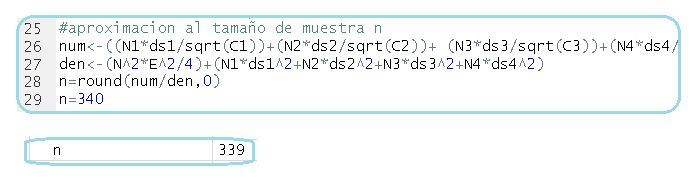
\includegraphics[scale=0.6]{Est3.JPG}
                    \caption{Modelo de Aproximación por estratos}
                    \label{etiqueta3}
            \end{figure}

        Así, se concluye que la aproximación de la muestra $n=339$ datos en total. 

            \subsection*{Número de encuestas por estrato}

        Es necesario ahora calcular el número de encuestas por estratos a partir de la aproximación de la muestra aleatoria estratificada.  Para ello se utilizará el siguiente modelo
    
           $$
           n_i=n\left ( \frac{\frac{N_i\sigma _i}{\sqrt{c_i}}}{\frac{N_1\sigma _1}{\sqrt{c_1}}+\frac{N_2\sigma _2}{\sqrt{c_2}}+...+\frac{N_L\sigma _L}{\sqrt{c_L}}} \right )
           $$ 

        Haciendo uso de RStudio se obtiene los siguientes resultados

        \begin{figure}[H]
                	\centering
                    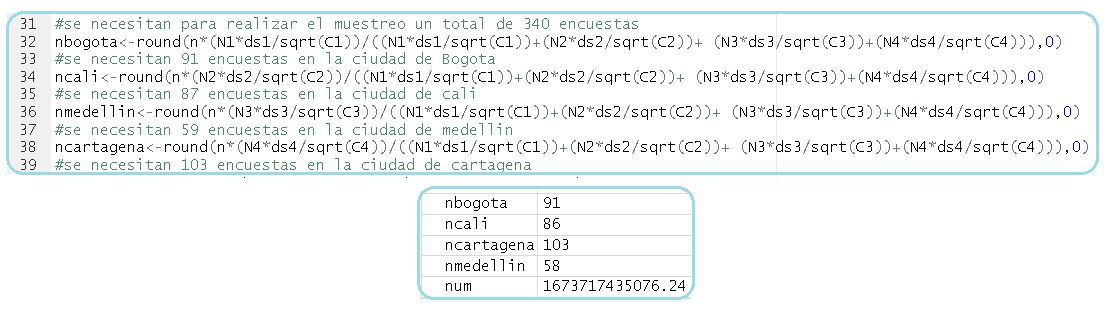
\includegraphics[scale=0.6]{Est4.JPG}
                    \caption{Muestreo Aleatorio Estratificado}
                    \label{etiqueta4}
            \end{figure}

        De esta manera, se concluye que, se necesitan 340 encuestas para realizar el muestreo aleatorio estratificado, de las cuales 91 encuestas son de la ciudad de Bogota, 86 encuestas son de la ciudad de Cali, 58 encuestas son de la ciudad de Medellín y 103 encuestas son de la ciudad de Cartagena.

        \subsection*{Gráfica}

            A continuación se presentan los comandos en RStudio para la construcción de las gráficas de las muestras de los estratos obtenidos en los apartados anteriores, además de sus correspondientes gráficas

            \begin{figure}[H]
                	\centering
                    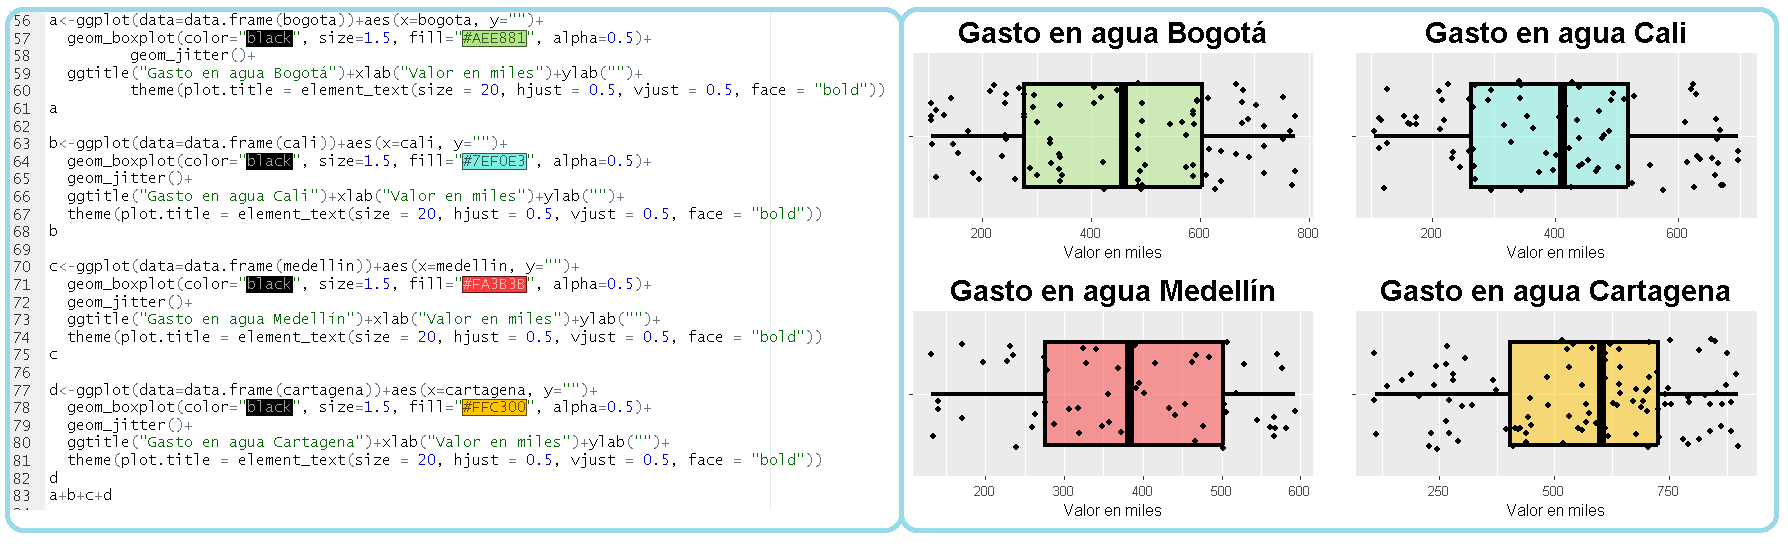
\includegraphics[scale=0.42]{Est6.JPG}
                    \caption{Gráfica Muestreo Aleatorio Estratificado}
                    \label{etiqueta5}
            \end{figure}

        En la gráfica se puede observar un diagrama de cajas y bigotes y a su vez de dispersión del gato de agua en miles de pesos para los estratos (ciudades) de Bogo´ta, Cali, Medellín y Cartagena. En el se puede observar los siguientes datos

        \begin{itemize}
            \item \textbf{Valor minimo:} Para Bogotá se sitúa sobre los 100 mil pesos, para Cali se sitúa sobre los 100 mil pesos, para Medellín se sitúa sobre los 160 mil pesos y para Cartagena se sitúa sobre los 120 mil pesos.
            \item \textbf{Cuartil 1:} Para Bogotá se sitúa sobre los 180 mil pesos, para Cali se sitúa sobre los 170 mil pesos, para Medellín se sitúa sobre los 270 mil pesos y para Cartagena se sitúa sobre los 335 mil pesos.
            \item \textbf{Cuartil 2 o media:} Para Bogotá se sitúa sobre los 460 mil pesos, para Cali se sitúa sobre los 410 mil pesos, para Medellín se sitúa sobre los 370 mil pesos y para Cartagena se sitúa sobre los 620 mil pesos.
            \item \textbf{Cuartil 3:} Para Bogotá se sitúa sobre los 600 mil pesos, para Cali se sitúa sobre los 510 mil pesos, para Medellín se sitúa sobre los 500 mil pesos y para Cartagena se sitúa sobre los 745 mil pesos.
            \item \textbf{Valor máximo} Para Bogotá se sitúa sobre los 775 mil pesos, para Cali se sitúa sobre los 690 mil pesos, para Medellín se sitúa sobre los 590 mil pesos y para Cartagena se sitúa sobre los 880 mil pesos.
        \end{itemize}

        De esta manera, se puede concluir que en las ciudades en las que hay ciudadanos que menos pagan por el servicio del agua son en Bogotá y en Cali, ý así mismo, la ciudad en la que hay ciudadanos que más pagan en agua es en Cartagena. Viendo los valores promedios, del menor al mayor, los ciudadanos que menos pagan al que más pagan en agua son Medellín, Cali, Bogotá y Cartagena.

        \subsection*{Estimacion de la media en el MAE} 

        A partir de cada uno de los estratos y la muestra tomada de cada estrato, la expresión que permite estimar la media en el muestreo aleatorio estratificado es la siguiente

            $$
             \bar{y}_{EST}=\frac{1}{N} \left [ N_1 \bar{y}_{1} + N_2 \bar{y}_{2} +...+ N_L \bar{y}_{L}\right ]
            $$
            
         Haciendo uso de la formula en RStudio se obtiene el siguiente resultado.
        
        \begin{figure}[H]
                	\centering
                    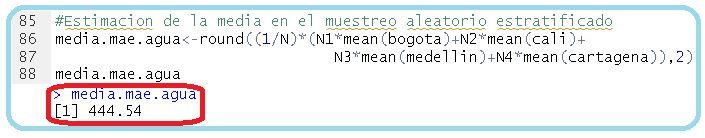
\includegraphics[scale=0.6]{Est7.JPG}
                    \caption{Estimacion de la media en el muestreo aleatorio estratificado}
                    \label{etiqueta6}
            \end{figure}
        Utilizando muestreo aleatorio estratificado, en promedio las familias pagan en agua un valor promedio de 444.54 mil pesos

    \subsection*{Calcular la varianza en el MAE}
    
       A partir de cada uno de los estratos y la muestra tomada de cada estrato, la varianza se puede calcular a partir de la siguiente sumatoria
        
    $$
    \hat{\sigma }{^2}_{media}=\frac{1}{N{^2}}\sum_{i=1}^{L}N_i{^2}\frac{S_i{^2}}{n_i}\left ( \frac{N_i-n_i}{N_i} \right )
    $$

        O bien sea

    $$
    \hat{\sigma }{^2}_{media}=\left ( \frac{1}{N{^2}} \right )\left [ N_1{^2}\frac{S_1{^2}}{n_1}\left ( \frac{N_1-n_1}{N_1} \right )+ N_2{^2}\frac{S_2{^2}}{n_2}\left ( \frac{N_2-n_2}{N_2} \right ) + N_3{^2}\frac{S_3{^2}}{n_3}\left ( \frac{N_3-n_3}{N_3} \right ) + N_4{^2}\frac{S_4{^2}}{n_4}\left ( \frac{N_4-n_4}{N_4} \right ) \right ]
    $$

    Haciendo uso de la formula en RStudio se obtiene el siguiente resultado
    
    \begin{figure}[H]
                	\centering
                    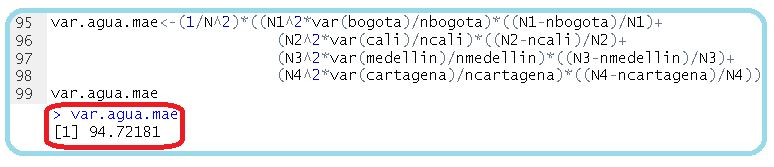
\includegraphics[scale=0.6]{Est8.JPG}
                    \caption{Varianza en muestreo aleatorio estratificado}
                    \label{etiqueta7}
            \end{figure}

        La varianza en el muestreo aleatorio estratificado es de 94.7 mil pesos.

        \subsection*{Intervalo de confianza para la media en el MAE}

        Los intervalos de confianza para la media en el Muestreo Aleatoria Estratificado se expresan a continuación

        \begin{itemize}
            \item \textit{Límite de confianza superior}

            $$
            L_{Sup}=\bar{y}_{EST}+2\left ( \sqrt{\frac{1}{N{^2}}\sum_{L}^{i=1}N_i{^2}\frac{S_i{^2}}{n_i}\left ( \frac{N_i-n_i}{N_i} \right )} \right )
            $$

            
            \item \textit{Límite de confianza inferior}

            $$
            L_{Inf}=\bar{y}_{EST}-2\left ( \sqrt{\frac{1}{N{^2}}\sum_{L}^{i=1}N_i{^2}\frac{S_i{^2}}{n_i}\left ( \frac{N_i-n_i}{N_i} \right )} \right )
            $$
            
        \end{itemize}

        Aplicando las formulas en RStudio se obtienen los siguientes resultados

        \begin{figure}[H]
                	\centering
                    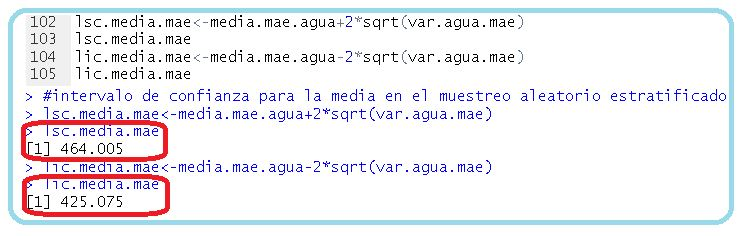
\includegraphics[scale=0.6]{Est9.JPG}
                    \caption{Intervalo de confianza para la media en el MAE}
                    \label{etiqueta8}
            \end{figure}

         \subsection*{Estimación del total en el MAE}

            La Estimación del total en el Muestreo Aleatorio Estratificado en estadística se utiliza para obtener una estimación del valor total de una variable de interés en una población, dividiendo la población en subgrupos o estratos y tomando una muestra de cada estrato. De esta manera, se presentaa la expresión que permite hallar la estimación total

            $$
            \hat{\tau }=[N1\bar{y}_1+N2\bar{y}_2+...+NL\bar{y}_L]
            $$

            Al aplicarlo en RStudio se obtiene el resultado de la estimación del total, el cual es de $3'062.839$ pesos.

             \begin{figure}[H]
                	\centering
                    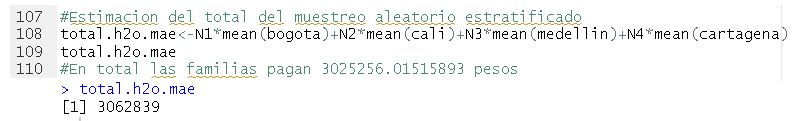
\includegraphics[scale=0.7]{estra2.JPG}
                    \caption{Estimación del total en MAE}
                    \label{etiqueta9}
            \end{figure}

         \subsection*{Estimación del error en el MAE}   

            La Estimación del Error en el Muestreo Aleatorio Estratificado en estadística es una técnica utilizada para reducir el error muestral al realizar un muestreo en una población dividida en grupos o estratos claramente identificables. En lugar de realizar un muestreo aleatorio simple en toda la población, se selecciona una muestra de cada estrato por separado. Esto permite obtener estimaciones más precisas y confiables al considerar las características específicas de cada estrato. La siguiente es la expresión que permite hallar la estimación de la varianza para el total en el MAE 

            $$
            \hat{\sigma }{^2}_{total}=\sum_{i=1}^{L}N_{i}{^2}\frac{S_{i}{^2}}{n_i}\left ( \frac{N_i-n_i}{N_i} \right )
            $$

            Para estimar el error, se debe hallar la raiz cuadrada de la estimación de la varianza para el total en MAE y multiplicarlo por 2, obteniendo así que

            $$
            \hat{e}_{total}=2\cdot \left ( \sqrt{\hat{\sigma }{^2}_{total}=\sum_{i=1}^{L}N_{i}{^2}\frac{S_{i}{^2}}{n_i}\left ( \frac{N_i-n_i}{N_i} \right )} \right )
            $$
            

            Y al aplicarlo en RStudio se obtiene que el error es de $133.417$ pesos.

                \begin{figure}[H]
                	\centering
                    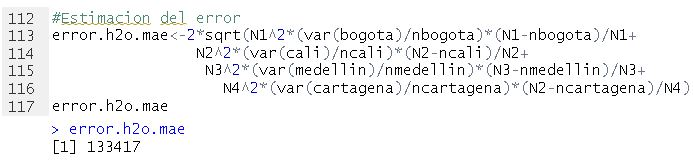
\includegraphics[scale=0.7]{estra3.JPG}
                    \caption{Error en en el MAE}
                    \label{etiqueta10}
            \end{figure}

         \subsection*{Intervalo de confianza para el total en el MAE}  

            El intervalo de confianza para el total en el Muestreo Aleatorio Estratificado en estadística se utiliza para estimar el valor total de una característica en una población, con un nivel de confianza determinado. Este método de muestreo se utiliza cuando la población se divide en estratos o subgrupos, y se selecciona una muestra aleatoria de cada estrato. Las expresiones que permiten hallarlo son las siguientes

            \begin{itemize}
            \item \textit{Límite  superior confianza}

            $$
            L_{SupT}=\hat{\tau }+2\left ( \sqrt{\sum_{i=1}^{L}N_i{^2}\frac{S_i{^2}}{n_i}\left ( \frac{N_i-n_i}{N_i} \right )} \right )
            $$

            
            \item \textit{Límite inferior de confianza}

            $$
            L_{SupT}=\hat{\tau }-2\left ( \sqrt{\sum_{i=1}^{L}N_i{^2}\frac{S_i{^2}}{n_i}\left ( \frac{N_i-n_i}{N_i} \right )} \right )
            $$
            
        \end{itemize}

        Al aplicarlo en RStudio se obtiene que en total las familias pagan entre $3'196.256$  y $2'9229.422$ pesos en servicios de agua.  

        \begin{figure}[H]
                	\centering
                    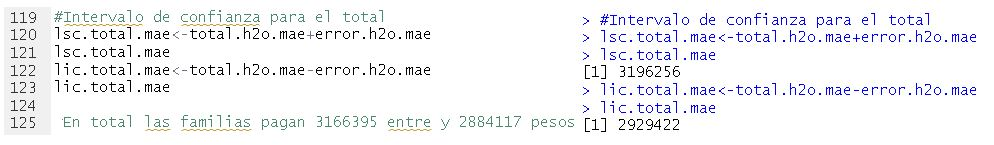
\includegraphics[scale=0.7]{estra4.JPG}
                    \caption{Error en en el MAE}
                    \label{etiqueta10}
            \end{figure}

         \subsection*{Estimacion de la Proporcion en el MAE}

         La estimación de la proporción en el muestreo aleatorio estratificado se utiliza para obtener una estimación precisa de una proporción en una población cuando se pueden identificar subgrupos o estratos claramente definidos. En este método de muestreo, la selección de elementos para formar la muestra se realiza por separado dentro de cada estrato, asegurando que ningún estrato quede sin muestrear. A continuación se presenta la expresión que permite Estimacion de la Proporcion en el Muestreo Aleatorio Estratificado

         $$
         \hat{p}_{est}=\frac{1}{N}\left [ N_1 \cdot \hat{p}_{1} + N_2 \cdot \hat{p}_{2} + ... +N_L \cdot \hat{p}_{L} \right ]
         $$

         Y ahora se presentará la estimación de la proporción de familias que pagan menos de 200.000 pesos en los diferentes estratos

            \begin{figure}[H]
                	\centering
                    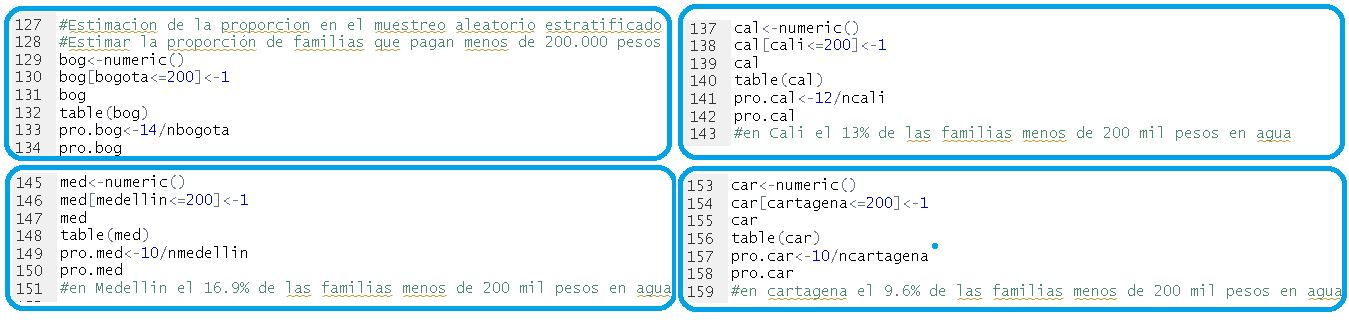
\includegraphics[scale=0.5]{estra5.JPG}
                    \caption{Estimacion de la Proporcion en el MAE en los distintos estratos}
                    \label{etiqueta11}
            \end{figure}

        De esta manera, se han obtenido la proporción de los distintos estratos $\hat{p}_{L}$, de los cuales se obtienen las conclusiones que el $16\%$ de las familias en Bogotá pagan menos de 200.000 pesos en servicios de agua, mientras que el $13\%$ de las familias en Cali pagan menos de 200.000 pesos en servicios de agua, el $16.9\%$ de las familias en Medellín pagan menos de 200.000 pesos en servicios de agua y el $9.6\%$ de las familias en Cartagena pagan menos de 200.000 pesos en servicios de agua. La estimación de la proporción MAE será la siguiente

         \begin{figure}[H]
                	\centering
                    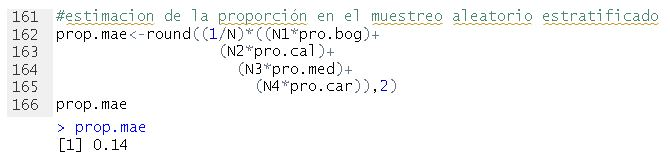
\includegraphics[scale=0.6]{estra6.JPG}
                    \caption{Estimacion de la Proporcion en el MAE en los distintos estratos}
                    \label{etiqueta12}
            \end{figure}

        Dicho resultado indica que en los cuatro estratos, es decir, en las 4 ciudades ya mencionadas, el $14\%$ paga menos de 200.000 pesos en servicios de agua. 

        \subsection*{Cota de error para la proporción en el MAE}

            La cota de error para la proporción en el Muestreo Aleatorio Estratificado es una medida de la variabilidad de las estimaciones de proporciones obtenidas a partir de una muestra estratificada. El objetivo del muestreo aleatorio estratificado es dividir la población en subgrupos o estratos claramente identificables y seleccionar una muestra aleatoria de cada estrato. Esto permite obtener estimaciones más precisas de las características de la población para cada subgrupo. La expresión que permite calcular la cota de error en el MAE es la siguiente

            $$
            e=2\left [ \sqrt{\frac{1}{N{^2}}\sum_{i=1}^{L}N_{i}{^2} \left ( \frac{\hat{p}_{i}\cdot \left ( 1-\hat{p}_{i} \right )}{n_1-1} \right ) \left ( \frac{N_i-n_i}{N_i} \right ) } \right ]
            $$
            
            Al aplicarlo en RStudio se obtienen que la cota de error es de $3,7\%$

            \begin{figure}[H]
                	\centering
                    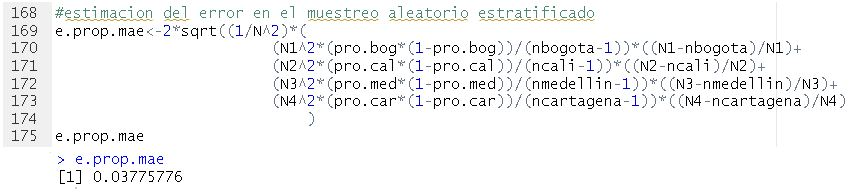
\includegraphics[scale=0.6]{estra7.JPG}
                    \caption{Estimacion del error en el MAE en los distintos estratos}
                    \label{etiqueta13}
            \end{figure}
            

        \subsection*{Intervalo de confianza para la proporción en el MAE}

        El intervalo de confianza para la proporción en el Muestreo Aleatorio Estratificado consiste en una técnica utilizada en estadística para estimar un rango dentro del cual se encuentra la proporción poblacional con cierta probabilidad. En el muestreo aleatorio estratificado, se seleccionan elementos de la muestra de forma separada dentro de cada estrato, asegurando que ningún estrato quede sin muestrear. A continuación se presentan las expresiones para calcularlos

             \begin{itemize}
            \item \textit{Límite  superior confianza}

            $$
            L_{SupP}=\hat{p}_{est}+2\left [ \sqrt{\frac{1}{N{^2}}\sum_{i=1}^{L}N_{i}{^2} \left ( \frac{\hat{p}_{i}\cdot \left ( 1-\hat{p}_{i} \right )}{n_1-1} \right ) \left ( \frac{N_i-n_i}{N_i} \right ) }\right ]
            $$

            
            \item \textit{Límite inferior de confianza}

            $$
            L_{SupP}=\hat{p}_{est}-2\left [ \sqrt{\frac{1}{N{^2}}\sum_{i=1}^{L}N_{i}{^2} \left ( \frac{\hat{p}_{i}\cdot \left ( 1-\hat{p}_{i} \right )}{n_1-1} \right ) \left ( \frac{N_i-n_i}{N_i} \right ) }\right ]
            $$
            
        \end{itemize}

        Al aplicarlo en RStudio se obtiene que el intervalo de confianza de la proporción es en MAE es de $18\%$  y $10\%$. 

        \begin{figure}[H]
                	\centering
                    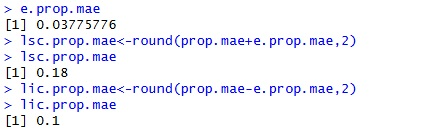
\includegraphics[scale=0.6]{estra8.JPG}
                    \caption{Intervalo de confianza para la proporción en el MAE}
                    \label{etiqueta14}
            \end{figure}

        \subsection*{Anexos}

         Link RScript: https://acortar.link/VQD0KP

    \bigskip
    

   
    
	    

\end{document}

